\chapter{Introducción}

%Introducción al TFG aquí: que vamos a hacer, que vamos a usar, objetivos a conseguir y finalidad. \todo{como en el resumen, habla de SDn como habilitador, incluso de 5G. Pero en estas afirmaciones tienes que poner referencias bibliográficas. Especialmente en la intro, que es la que motiva todo lo demás.}
%\todo{habla un poco de qué es SDN, resumido, y openflow. Luego comenta qué se hará: el diseño de los mecanismos, y luego un ejemplo práctico en el que se adapta una red corporativa existente...}

En este Trabajo Fin de Grado vamos a diseñar e implementar una red de ordenadores que se configure de forma automática y dinámica sin necesidad de intervención de un operador. La red será de tipo corporativo y tendrá la mínima intervención una vez desplegada inicialmente. Esta red hará uso de Redes Definidas por Software, tecnología que está revolucionando el campo de las redes de ordenadores por las grandes ventajas que ofrece y su rápida evolución en los últimos años. \cite{alma991014010918704990}

Para el desarrollo de este tipo de redes utilizaremos librerías y entornos de trabajos de software libre como OpenFlow. OpenFlow es un protocolo de comunicación entre switches y controladores de red abierto \cite{OpenNetw57:online} y es usado por las redes definidas por software como mecanismo de control sobre las operaciones de red, permitiendo programar aplicaciones que controlen de forma centralizada como se mueven, procesan o modifican los paquetes que viajan por la red.

En una primera parte de esta memoria vamos a revisar el estado de la tecnología y las herramientas de las que vamos a disponer. Luego analizaremos los requisitos que tiene que cumplir la red a desarrollar y los objetivos a alcanzar. Dichos objetivos serán extraídos de los requisitos del problema a resolver.

Más tarde explicaremos el proceso de diseño, implementación y pruebas de esta red y las dificultades encontradas durante dicho proceso. Por último hablaremos de posibles ampliaciones al proyecto y trabajos futuros.

Toda esta memoria, así como el código generado en este proyecto tiene licencia MIT y está disponible en \url{https://github.com/jscoba/ryu-vlan-tfg}


\chapter{Estado de la tecnología.}

Para poder desarrollar el trabajo necesitamos conocer previamente el estado actual de las redes de ordenadores así como los tipos de herramientas que necesitaremos para poder completar el desarrollo de la propuesta.

Haremos un repaso del estado de madurez de las redes definidas por software y conoceremos un poco su historia reciente. Más adelante identificaremos los tipos de herramientas que necesitamos y haremos una pequeña comparativa entre las opciones disponibles, seleccionando las más convenientes para nuestro proyecto.

%Hacer un análisis de las herramientas que vamos a utilizar. y un poco de historia a las SDN

\section{\acrshort{sdn}: Redes definidas por software}

\subsection{Qué son las SDN.}

Las redes definidas por software (Software Defined Networks, en inglés) son un tipo de redes de ordenadores con un enfoque distinto a las redes tradicionales en el que se separan los planos de control y de datos, tradicionalmente integrados dentro de un mismo dispositivo (hardware o software) para permitir un mejor control de los flujos de paquetes en la red y dotar a la misma de capacidad de análisis y procesamiento de paquetes, tareas para las que se requiere hasta ahora dispositivos y softwares específicos.\cite{alma991014010918704990}.
%\todo{En las definiciones, cuando hables de una tecnología completa, etc., pon una referencia bibliográfica. Aprovecha que hay muchos libros en la biblioteca de la UGR. Busca en google esa referencia para bibtex, por si estuviera ya indexada en alguna base d edatos.}.

Para entender bien lo novedoso de este tipo de redes necesitamos conocer en detalle que son los planos de control y de datos y como, separándolos, podemos aprovechar las ventajas que ofrece esta nueva arquitectura de red 

\begin{figure}[h!]
    \centering
    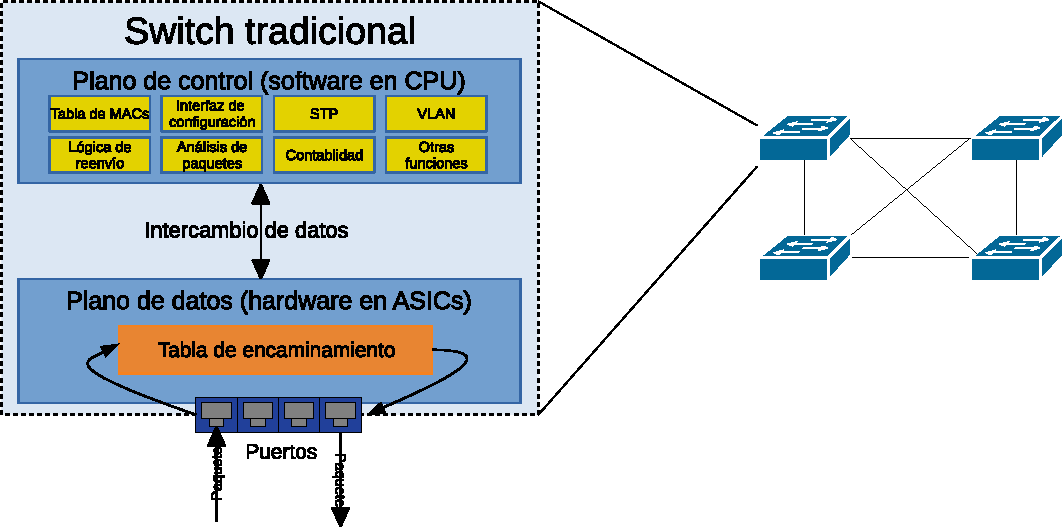
\includegraphics[width=\textwidth]{imagenes/figuras/Switch tradicional.pdf}
    \caption{Figura de planos de control y de datos}
    \label{fig:planos_red_tradicional}
\end{figure}



Como podemos ver en la figura \ref{fig:planos_red_tradicional} podemos dividir en dos planos principales a los dispositivos de red (routers y switches). Un \textbf{plano de datos} encargado de mover los paquetes que entran desde los distintos puertos siguiendo unas instrucciones (tablas de encaminamiento) y un \textbf{plano de control} encargado de calcular dichas tablas, dependiendo de las características del paquete recibido (puerto de origen, cabeceras del paquete, etc). Estos planos se encuentran dentro del mismo dispositivo y están altamente acoplados, teniendo que ser el plano de control consciente del sistema que trabaja por debajo. Normalmente el plano de datos está implementado directamente en circuitos físicos, sea mediante \acrshort{asic2}'s\footnote{Application-Specific Integrated Circuit, Circuitos hardware con una función muy específica, lo que les aporta una gran velocidad y un bajo consumo energético.} o cualquier otro tipo de hardware especializado. Este acoplamiento hace que el plano de control esté definido de forma cerrada por el fabricante del equipo y limitado a lo que el fabricante haya integrado.


El hecho de que los planos de control y de datos (y en general los equipos de red) sigan un esquema de desarrollo cerrado fijado por el fabricante hace que no se puedan actualizar las redes a los avances que la tecnología está sufriendo estos días. En los equipamientos de red esto se acentúa ya que suelen ser equipos muy caros y con una vida media de muchos años. Al final acabamos con un ecosistema de red que no puede adaptarse a las nuevas necesidades por si mismos, sino que una vez comprado e instalado es (casi) imposible actualizar la red y sus equipos y añadir nuevas funcionalidades.

Existe además una relación entre los problemas de seguridad y esta falta de flexibilidad por parte de la red. Si se descubre alguna vulnerabilidad en algún protocolo de red estamos casi seguros de que no vamos a poder mitigarlo sin tener que pagar por un equipo nuevo que incluya los parches de seguridad necesarios. Además, como el equipo de red funciona como un todo, las actualizaciones y nuevas funcionalidades tienen un ciclo de desarrollo muy lento, pues es necesario crear (o modificar) las funciones del equipo de red teniendo en cuenta todos los aspectos (software y hardware) del equipo (y en definitiva, sacar un nuevo modelo). 

Aunque se han hecho avances en la modularidad de los equipos de red (utilizando por ejemplo sistemas operativos actualizables como iOS o RouterOS) seguimos teniendo un esquema cerrado en el que los equipos de diferentes proveedores no son compatibles a la perfección entre sí.


\begin{figure}[h!]
    \centering
    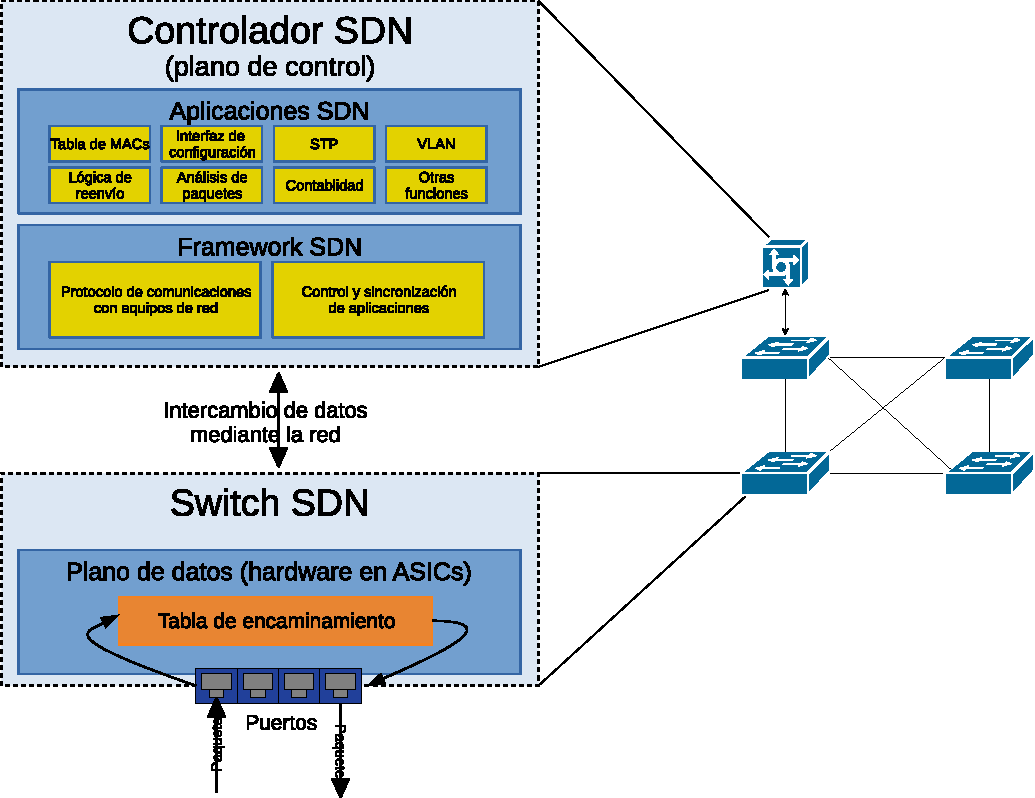
\includegraphics[width=\textwidth]{imagenes/figuras/Switch sdn.pdf}
    \caption{Figura de planos de control y de datos en SDN}
    \label{fig:planos_red_sdn}
\end{figure}

La gran revolución que presentan las Redes Definidas por Software es la separación entre el plano de control y el plano de datos de los dispositivos de la red (Figura \ref{fig:planos_red_sdn}). Hardware especializado sigue encargándose de reenviar (o no) los paquetes que llegan a los distintos puertos del dispositivo, pero es un sistema externo el que se encarga de decidir donde se tienen que enviar los paquetes (calcular las tablas de encaminamiento).

En una Red Definida por Software existe la figura del \emph{controlador de la red}, un dispositivo (normalmente un servidor) que ejecuta la lógica de la red y establece las distintas tablas y rutas que los switches tienen que seguir en el momento en el que tienen que procesar un paquete de datos. Este controlador, al ser una aplicación, puede ejecutarse en un servidor físico, una máquina virtual, agrupaciones de servidores (clusters) o incluso en servidores en la nube, proporcionando un control centralizado de lo que ocurre en la red. Además permite una comunicación del estado de la red con otras aplicaciones, lo que sirve para, si así se desea, optimizar la red en cuestión a las distintas necesidades que las aplicaciones que se ejecutan sobre ellas tengan.

Hasta ahora, la aparición de un nuevo protocolo o un nuevo problema a resolver ha conllevado iniciar un nuevo proceso de diseño de un nuevo modelo de switch o router (o sistema operativo) para implementar la solución necesaria (añadir soporte de VLAN, firewall, compatibilidad con nuevos protocolos como IPv6, etc). Mediante el enfoque de las SDN añadir nuevas funcionalidades es tan sencillo como escribir una aplicación software que resuelva el problema. Al ser un producto únicamente software este sigue su modelo de desarrollo, mucho más ágil que el desarrollo hardware y, normalmente, más barato.


\subsection{Las primeras SDNs.}

La idea de separar los planos de control y de datos apareció en 2004 mediante una propuesta de la \acrshort{ietf} publicada como RFC3746\cite{rfc3746}. Esta primera aproximación no fue bien recibida por los fabricantes de equipos de red debido a los grandes daños que podría causar un fallo en el plano de control. No fue hasta 2008 que se retomó la idea de separar los planos de control y datos de las redes de ordenadores con la propuesta de la Universidad de Stanford \cite{openflowstanford} de una \acrshort{api} \footnote{Application Programming Interface, una especificación de funciones e interfaces para que distintos programas se comuniquen entre si.} para implementar redes SDN, OpenFlow. A partir de ese momento empresas como Google \cite{hoelzlet78:online}, HP o NTT empezaron a desarrollar sus propias implementaciones de SDN, bien usando OpenFlow o diseñando sus propias APIs y protocolos. Un momento de especial interés es 2011 cuando se funda la Open Networking Fundation \cite{OpenNetw57:online}, una organización formada por operadores de red dedicada a promover las redes definidas por software y a estandarizar el protocolo OpenFlow. 

\subsection{Protocolos y estandarización.}

Aunque en este documento hemos hablado de SDN y de OpenFlow cabe destacar que no son lo mismo. SDN es un concepto de redes programables que ejecutan aplicaciones de control para gestionar el tráfico de una red. Como concepto que es se trata de una forma de diseñar redes, no de un programa específico para hacer esto. OpenFlow es un protocolo abierto de comunicación entre dispositivos de red y controladores de la misma que permiten el despliegue de redes SDN. Es, en si mismo, una especificación de una API para lograr el objetivo de crear redes definidas por software. Sin embargo existen otros protocolos (propietarios, de distintos fabricantes) que se utilizan para implementar SDN. Ejemplos de estos protocolos y arquitecturas son Cisco DNA de Cisco\cite{CiscoDNA47:online}, NETCONF (basado en XML)\cite{rfc6022} o OVSDB de OpenVSwitch \cite{OpenvSwi96:online}.

Sin embargo OpenFlow es el protocolo de comunicación con dispositivos de red para SDN más popular, debido a su carácter libre y al potente apoyo que recibe por parte de la Open Networking Foundation. Además, es soportado por una gran cantidad de fabricantes de equipos (incluso los que tienen sus propios protocolos de SDN) como Cisco, Mikrotik, HP, Jupyter Networks, etc.

El proceso de estandarización de OpenFlow está liderado por la Open Networking Foundation, que publica periodicamente nuevas versiones del protocolo, siendo la última versión la 1.5 \cite{SDNTechn21:online}. A partir de la especificación del protocolo hay diversas implementaciones del mismo (algunas propietarias) pero que son capaces de comunicarse con los dispositivos de red (hardware o virtualizados) que se adhieran al protocolo. Algunas de estas implementaciones son: OpenDayLight, RYU, NOX o Beacon \cite{ListofOp48:online}.

\subsection{Comparación con redes tradicionales: ventajas e inconvenientes.}

%Comparar facilidad de uso, despliegue, costes operativos, etc.

A continuación vamos a realizar una comparativa entre una red tradicional y una red definida por software, resaltando las posibles ventajas que puede tener una respecto a la otra dependiendo del escenario en el que nos encontremos.

Podemos empezar comentando que dependemos del escenario para elegir una arquitectura de red frente a la otra. Las SDN son por lo general más complejas que una red tradicional en escenarios donde tenemos muy pocos dispositivos, por ejemplo en una red doméstica de área local en la que no tenemos que hacer ningún tipo de ingeniería del tráfico. Sin embargo en redes corporativas donde tenemos gran cantidad de dispositivos, usuarios y requerimientos específicos nos puede ser de gran ayuda plantearnos diseñar la red con la arquitectura de SDN. Un ejemplo de esto es cuando tenemos una única infraestructura de red para ofrecer servicios diferenciados (DiffServ), en el que por una única red viajan paquetes de ordenadores, teléfonos VoIP, cámaras de seguridad, impresoras, servidores, etc. En una red tradicional podemos conseguir este tipo de red configurando manualmente cada uno de los switches y routers para poder conseguir el comportamiento esperado. Esta tarea se hace especialmente tediosa en redes muy grandes y en redes dinámicas, en las que los servicios y los requisitos cambian continuamente a medida que pasa el tiempo (empresas que se amplían, nuevos servicios, renovación de equipos, etc).

Con una red definida por software todas las tareas de administración de la red están centralizadas en el controlador y, ante la aparición de nuevos requisitos de la red, solo hay que modificar el comportamiento del mismo (o escribir uno nuevo) para poder adaptar la red a las nuevas necesidades. Además permite la integración tanto de nodos de red hardware como software, por lo que la gestión de infraestructuras virtualizadas (sea en un centro de datos propio o en la nube pública) se hace mucho más sencilla.

En una comparativa de este tipo no podemos dejar de hablar de los costes económicos de los distintos tipos de redes. Especialmente vamos a comparar los costes de capital (compra de equipos) y los costes operativos (coste de funcionamiento), también conocidos por sus siglas en inglés \acrshort{capex} y \acrshort{opex}.

\begin{itemize}
    \item CAPEX: Son los gastos de adquirir bienes en una empresa. En el contexto en el que estamos hablando ahora mismo sería el coste de los equipos y el despliegue inicial de la red. Estos son similares tanto en una red tradicional como en una red definida por software, pudiendo ser incluso menores en estas últimas. Esto se debe a que los equipos de diferentes fabricantes son compatibles entre sí, por lo que no estamos atados a un único fabricante y podemos elegir los dispositivos más competitivos económicamente.
    \item OPEX: Son los gastos de operación de una empresa. Hablando de redes son los costes derivados de mantener la red operativa y actualizada para que ofrezca el rendimiento deseado. En una red definida por software estos gastos son menores. Esto se debe a que son más fáciles de gestionar (hace falta menos personal) y a que son mucho más modulares y expandibles que las redes tradicionales. Un ejemplo de esto es que, si queremos añadir una nueva funcionalidad a la red (sin tener que adquirir nuevo equipamiento) la configuración de una red tradicional es mucho más lenta, por lo que la operación se extenderá más en el tiempo que con una SDN, con su correspondiente pérdida de dinero derivada de no tener la red al 100\% de su capacidad durante un tiempo. Además no tenemos por qué estar sometidos a los esquemas de licencias de los fabricantes de red (o al menos de un único fabricante) habiendo, al ser un mercado estandarizado e interoperable, mayor oferta de proveedores y por tanto menor coste.
\end{itemize}

Podemos resumir la comparativa entre redes tradicionales y redes definidas por software de la siguiente manera:

\begin{itemize}
    \item Ventajas de las SDN frente a las redes tradicionales:
    \begin{itemize}
        \item Gestión más sencilla.
        \item Fácilmente expandibles.
        \item No están limitadas a un único proveedor de equipos.
        \item Permiten un mayor aprovechamiento de la infraestructura existente.
        \item Reducen los costes operativos de la empresa.
        \item Aumento del rendimiento y fácil optimización.
        \item Permiten el reaprovechamiento de equipos existentes, lo que reduce costes.
    \end{itemize}
    \item Desventajas de las SDN frente a las redes tradicionales:
    \begin{itemize}
        \item Son más complejas de diseñar e implementar.
        \item Requieren una infraestructura de servidores para funcionar.
        \item No merecen la pena en redes simples.
        \item Es una tecnología en constante evolución, por lo que aún tiene mucho margen de mejora.
    \end{itemize}
\end{itemize}

En definitiva podemos ver que las redes definidas por software presentan unas ventajas nada despreciables frente a las redes tradicionales.

\section{Comparativa y elección de herramientas.}

\subsection{Sistema de emulación de redes. Laboratorio virtual}

La primera herramienta que necesitamos para desarrollar nuestro proyecto es un software capaz de emular redes de ordenadores para poder realizar todas las pruebas necesarias sobre nuestro sistema. Además, este software debe ser compatible con OpenFlow para poder implementar SDN y no una simple red tradicional. Para esto último tenemos muchas herramientas como PacketTracer de Cisco o CORE Network Emulator (entre muchos otros). Sin embargo ninguna de estas herramientas permiten emular switches compatibles con OpenFlow, por lo que no nos son de utilidad.

Revisando las opciones disponibles nos encontramos con 2 herramientas candidatas: NS3 \cite{ns3adisc22:online} y Mininet\cite{MininetA12:online}.

NS3 es un software de simulación de redes libre que permite simular redes de ordenadores en un ordenador. Mininet es un software de emulación de redes también libre que utiliza tecnologías de virtualización de Linux para generar nodos virtuales en un ordenador. En la tabla \ref{tab:mininet_ns3} vamos a comparar sus características principales.

\begin{table}[h!]
    \centering
    \begin{tabular}{|c|c|c|}
    \hline
        Característica & Mininet & NS3  \\
    \hline
         Tipo de software & Emulación & Simulación\\
    \hline
        Licencia & BSD & GPLv2 \\
    \hline
        Lenguaje & Python & C++ \\
    \hline
        Soporta OpenFlow & Si & Si \\
    \hline
        Soporta WiFi & Si & Si \\
    \hline
        Repaldado por & ONF  & Indenpendiente \\
    \hline
    \end{tabular}
    \caption{Comparativa entre Mininet y NS3}
    \label{tab:mininet_ns3}
\end{table}

Debido a su soporte por parte de la Open Networking Foundation y a que se utiliza creando scripts en python vamos a elegir \textbf{Mininet} (en su versión compatible con wifi) como software de laboratorio de pruebas para el desarrollo de nuestra red inteligente.

\subsection{Framework del controlador OpenFlow}

Como ya hemos comentado anteriormente OpenFlow es la especificación de un protocolo de comunicación entre un controlador de una SDN y el plano de datos de un switch compatible. Necesitamos elegir un framework de trabajo que nos permita escribir nuestras propias aplicaciones para la red e implemente OpenFlow para la comunicación con los switches.

En el mercado existen gran variedad de soluciones que resuelven este problema. Como estamos en un entorno académico vamos a centrarnos en las opciones que sean Open Source (código libre), pues, generalmente, presentan una mejor documentación y tienen soporte dado por una comunidad global. Al ser productos libres es muy probable que si tenemos algún problema alguien lo haya tenido ya y la solución se encuentre en internet publicada.

Entre las opciones más maduras tenemos: Ryu, OpenDayLight y POX.

En la tabla \ref{tab:comparativa_frameworks} vamos a comparar las características más reseñables de estos tres proyectos.

\begin{table}[h!]
    \centering
    \begin{tabular}{|c|c|c|c|}
    \hline
        Característica & RYU & OpenDayLight & POX  \\
    \hline
        Versión de OpenFlow & 1.5 & 1.3 & 1.0 \\
    \hline
        Licencia & Apache & Eclipse & Apache \\
    \hline
        Lenguaje & Python 3 & Java  & Python 2\\
    \hline
        Documentación disponible & Bastante & Mucha  & Suficiente \\
    \hline
        Último commit a su repositorio & 2020 & 2020  & 2017 \\
    \hline
        Desarrollado por & FaucetSDN  & Linux Foundation  & Nicira Inc.\\
    \hline
    \end{tabular}
    \caption{Comparativa entre frameworks OpenFlow}
    \label{tab:comparativa_frameworks}
\end{table}

Por su soporte de OpenFlow, su documentación y estar programado en Python utilizaremos \textbf{Ryu} como framework de desarrollo del controlador de nuestra SDN.

\subsection{Otras herramientas}

Además del laboratorio de pruebas y el framework de OpenFlow necesitaremos algunas herramientas adicionales para poder diseñar, implementar y probar nuestra red. Primeramente necesitaremos un software de análisis de tráfico que nos ayude a ver el camino que los paquetes siguen en nuestra red. La herramienta \emph{de facto} en el desarrollo de redes bajo el sistema operativo Linux es \textbf{Wireshark}, que nos permite capturar y analizar paquetes desde cualquier interfaz a la que tengamos acceso. Mininet nos proporciona interfaces virtuales que nos permiten escuchar cada uno de los enlaces que estamos virtualizando.

También nos hace falta alguna manera de generar tráfico en nuestra red para así poder estimar su rendimiento. Para esto vamos a utilizar dos herramientas diferentes. Por un lado tenemos \textbf{iperf}, que nos permite generar un flujo de paquetes controlando el ancho de banda que queremos consumir (o generando todo el tráfico que pueda y así probar a sobrecargar los enlaces y con ello, finalmente, la red). Utilizaremos adicionalmente el generador de tráfico \textbf{D-ITG}, una herramienta que nos permite simular distintos patrones de tráfico como VoIP, juegos online, tráfico HTTP, etc. Lo que nos permitirá mejorar nuestra capacidad de análisis sobre el rendimiento de la red haciendo una simulación de carga de trabajo que se ajuste mejor a los requisitos.


%\chapter{Pruebas de herramientas: red sencilla}
%MOVER ESTE CAPITULO A OTRA PARTE (SI LLEGA A HACERSE).
%Una simple topo linear de mininet con un controlador de ryu.

%\section{Comparativa con redes convencionales.}
